%%%%%%%%%%%%%%%%%%%%%%%%%%%%%%%%%%%%%%%%%
\section{The electricity model}
\label{sec:CodeDocElec}

The model presented in this chapter is a transposition of the model created by Paul van Baal and Reinier Verhoog and first created by Paul van Baal for his master thesis \citep{van2016business}. The model has also been further improved to look into the effect of a strategic reserve in a hybrid system dynamics - agent based model version \citep{van2019effectiveness}. In this report, the model, which was a system dynamics model and then a hybrid model, is turned into an agent based model. This report is the ODD presentation of that model \citep{grimm2010odd}. All equations and additional details are in the appendices.

%%%%%%%%%%%%
\subsection{Purpose of the model}
\label{ssec:purpose}

The purpose of this model is to simulate the Swiss electricity system. This includes the spot market, international trade with neighbouring countries, and investments. This constitutes what is considered to be the simplest electricity model (SMel). In future iterations of the model, depending on the goals of the research, the model can be extended to consider the presence of demand side management, batteries, prosumers or a strategic reserve.

%%%%%%%%%%%% end of subsection

%%%%%%%%%%%%
\subsection{Entities, state variables and scales}
\label{ssec:entities}

There are four types of agents within the model: the market operator, the firms (or investors), the supply agents and the demand agents. The market operator is the agent that is in charge of the spot market, making sure everything is going well. The firms are the agents that own the power plants and other assets present in the model. They are in control of the  power plants. The demand agents are the agents that buy electricity. This includes the inflexible demand (which is based on a  historical scenario), and demand created by hydro-pumping power and international trading.

%There are two types of agents within the model: the agents which are in charge of taking care of the electricity market and the assets which represent the physical infrastructure and which produce electricity.

The firms are characterised by the following attributes: assets owned, electricity supplied, planned assets, retired assets and constructed assets. The supply agents can either be the power plants (assets), they can be long term contracts with France, or they can be the net transfer capacities from the different border countries. Each has a different set of attributes. The assets are characterised by the following attributes: owner, technology type, installed capacity, age, lifespan, capital costs, annual fixed costs, variable costs and utilisation factor. Additionally, depending on the technology type, some power plants have more parameters. For example, the thermal power plants, the nuclear power plants and the waste power plants all have a fuel cost. The thermal power plants also have an emission attribute. The nuclear power plants have attributes related to their maintenance requirements: maintenance month and maintenance time. Waste, hydro and hydro-pumping assets have attributes related to their reservoirs: reservoir level and maximum reservoir level. Hydro-pumping assets have an efficiency attribute related to their pumping efficiency.

The technology types are limited to: solar, wind, hydro power, hydro-pumping power, run of river, thermal, nuclear and waste. The firms can only invest in solar, wind and thermal technologies as it is considered that other technologies are already maxed out in Switzerland or they cannot be used to produce significantly more electricity.

%The actors are provided as follows: the market operator, the firms, the supply agents and the demand agents. The market operator is the agent that runs the spot market. The firms represent the investors that have the capacity to invest for new generation capacity. They also have to decide whether to keep plants online, if they should be mothballed or dismantled. The supply agents are the plants themselves but they can also include foreign countries. Finally, the demand agents create the electricity demand that represents the demand in Switzerland but also the demand of hydropower pumping plants.

%%%%%%%%%%%% end of subsection

%%%%%%%%%%%%
\subsection{Process overview and scheduling}
\label{ssec:process}

The model runs along two different scales, highlighting two parts of the model. The first part is the spot market, running on an hourly basis. It consists of all the actions related to the spot market including all of the inputs, the calculation of the demand, the calculation of the spot price, the distribution of the money and electricity when the equilibrium is found and the update of the NPV for all of the agents (that is later used for investments).

The second part is related to the investments that the firms can perform. This happens monthly. These are actions that are related to the firms. They decide whether to invest in new assets. They also decide whether they should reinvest in their current assets by extending their lifetimes or shuttering them temporarily or definitively. Then there are additional measures that include the end of life actions that occurs when an asset has reached its lifetime. It also includes scenario based events such as the closing of nuclear power plants according to a politically determined timeline.

%%%%%%%%%%%% end of subsection

%%%%%%%%%%%%
\subsection{Design concepts}
\label{ssec:design}

%%
\paragraph{Basic principles}
%Which general concepts, theories, hypotheses, or modeling approaches are underlying the model?s design? Explain the relationship between these basic principles, the complexity expanded in this model, and the purpose of the study. How were they taken into account? Are they used at the level of submodels (e.g., decisions on land use, or foraging theory), or is their scope the system level (e.g., intermediate disturbance hypotheses)? Will the model provide insights about the basic principles themselves, i.e., their scope, their usefulness in real-world scenarios, validation, or modification (Grimm, 1999)? Does the model use new, or previously developed, theory for agent traits from which system dynamics emerge (e.g., ?individual-based theory? as described by Grimm and Railsback [2005; Grimm et al., 2005])?

The model is, in essence, a simple supply and demand model where electricity is demanded and supplied. The main added element is that instead of resolving this supply and demand every week or year as it has been done in past models, it is done on an hourly basis.

%%
\paragraph{Emergence}
%What key results or outputs of the model are modelled as emerging from the adaptive traits, or behaviours, of individuals? In other words, what model results are expected to vary in complex and perhaps unpredictable ways when particular characteristics of individuals or their environment change? Are there other results that are more tightly imposed by model rules and hence less dependent on what individuals do, and hence ?built in? rather than emergent results?

The main outputs of the model relate to the energy mix that is needed to meet the Swiss electricity demand. The investments, their type and amount are also of interest for the purpose of the study and should emerge from the needs to supply electricity.

%%
\paragraph{Adaptation}
%What adaptive traits do the individuals have? What rules do they have for making decisions or changing behaviour in response to changes in themselves or their environment? Do these traits explicitly seek to increase some measure of individual success regarding its objectives (e.g., ?move to the cell providing fastest growth rate?, where growth is assumed to be an indicator of success; see the next concept)? Or do they instead simply cause individuals to reproduce observed behaviors (e.g., ?go uphill 70\% of the time?) that are implicitly assumed to indirectly convey success or fitness?

There is no real adaptation programmed in this model beyond agents deciding on whether to discontinue their current assets and whether to invest in current or new ones.

%%
\paragraph{Objectives}
%If adaptive traits explicitly act to increase some measure of the individual?s success at meeting some objective, what exactly is that objective and how is it measured? When individuals make decisions by ranking alternatives, what criteria do they use? Some synonyms for ?objectives? are ?fitness? for organisms assumed to have adaptive traits evolved to provide reproductive success, ?utility? for economic reward in social models or simply ?success criteria? (note that the objective of such agents as members of a team, social insects, organs ? e.g., leaves ? of an organism, or cells in a tissue, may not refer to themselves but to the team, colony or organism of which they are a part).

The objectives for the market operator is that there be a balanced spot market. The objective for the firms is to make as much money as possible. The objective of the supply agents is to supply as much energy as possible. The objective of the demand agents is to have their demand met. 

%%
\paragraph{Prediction}
%Prediction is fundamental to successful decision-making; if an agent?s adaptive traits or learning procedures are based on estimating future consequences of decisions, how do agents predict the future conditions (either environmental or internal) they will experience? If appropriate, what internal models are agents assumed to use to estimate future conditions or consequences of their decisions? What tacit or hidden predictions are implied in these internal model assumptions?

The firm agents have to use prediction for the investments. They forecast the price of electricity for the next year, two years and five years based on historical data for each technology considered. This is then used in the profitability check and the Net Present Value (NPV) by the firms for their respective assets or future investments.

%%
\paragraph{Sensing}
%What internal and environmental state variables are individuals assumed to sense and consider in their decisions? What state variables of which other individuals and entities can an individual perceive; for example, signals that another individual may intentionally or unintentionally send? Sensing is often assumed to be local, but can happen through networks or can even be assumed to be global (e.g., a forager on one site sensing the resource lev- els of all other sites it could move to). If agents sense each other through social networks, is the structure of the network imposed or emergent? Are the mechanisms by which agents obtain information modelled explicitly, or are individuals simply assumed to know these variables?

The sensing of the actors is limited. Only the firms have sensing. They have a clear and full understanding of the performance of their assets. This includes the costs involved, the electricity generated and sold, and for some technologies, the reservoir related values. For investments, actors only inform their investment potential based on what assets are present in the system and the overall price of electricity. They do not have knowledge of other firm's assets in construction or planned. This can therefore lead to periodical supply surplus.

%%
\paragraph{Stochasticity}
%What processes are modeled by assuming they are random or partly random? Is stochasticity used, for example, to reproduce variability in processes for which it is unimportant to model the actual causes of the variability? Is it used to cause model events or behaviors to occur with a specified frequency?

Most of the model is deterministic. Some outages can occur randomly for each of the plants. Scenarios also provide some stochasticity to the simulation.

%%
\paragraph{Observation}
%What data are collected from the ABM for testing, understanding, and analyzing it, and how and when are they collected? Are all output data freely used, or are only certain data sampled and used, to imitate what can be observed in an empirical study (?Virtual Ecologist? approach; Zurell et al., 2010)?

The model produces a large amount of data. Not all of it is necessary for testing, understanding and analysis. Some of the data needs to be collected to feed the policy process model. The agents in the policy process based their decision based on what is going on with a set of key performance indicators in the electricity model. Beyond this, the interest for understanding and analysis is mostly focused on the electricity prices, the number of outages (if any), the supply mix, and the trade with foreign countries. Depending on the study being performed, the amount of investment is also of interest along with the type of investment and measures related to the goals of the Energy Strategy 2050.

%%%%%%%%%%%% end of subsection

%%%%%%%%%%%%
\subsection{Initialisation}
\label{sec:initialisation}

The model is initialised with values from 2018 for all of the assets that are present in the model. This includes the 2018 Swiss electricity power plants distribution and costs. The initialisation state is always the same for all simulations. All the values considered are informed on the Swiss electricity sector directly.

%%%%%%%%%%%% end of subsection

%%%%%%%%%%%%
\subsection{Input data}
\label{ssec:inputData}

There are a lot of input data required to simulate the electricity system. The data used to run the model is given below:

\begin{itemize}
\item Asset investment (type, sizes and costs) 
\item The gas prices for thermal power plants (scenario based)
\item The emission prices for thermal power plants (scenario based)
\item The water inflow in Swiss reservoirs for hydro power plants yearly and hourly (scenario included)
\item The waste inflow in Swiss waste management facilities yearly (scenario based)
\item The price of nuclear fuel (scenario based)
\item The amount of solar radiation hourly (based on the years 2015, 2016 and 2017)
\item The amount of wind hourly (based on the years 2015, 2016 and 2017)
\item The amount of run of river water (based on the years 2010, 2011, 2012, 2013 and 2014)
\item The average hourly electricity price in France, Germany and Italy (based on the years 2015, 2016 and 2017)
\item The average border capacity (import and export) with France, Germany and Italy (based on the years 2015, 2016 and 2017)
\end{itemize}

%%%%%%%%%%%% end of subsection

%%%%%%%%%%%%
\subsection{Submodels}
\label{sec:submodel}

There is a large number of submodels that are used to simulate the Swiss electricity market. They are all detailed qualitatively within this section. The equations used are present in the appendix for each submodel.

\begin{enumerate}
\item The spot market
\item The electricity price forecast
\item The profitability calculation
\item The NPV calculation
\item The end of life actions
\item The international trading
\item The demand aspect of storage in the model
\end{enumerate}

%%
\paragraph{The spot market}

The spot market is at the centre of the model. Its role is to match supply with demand. Some of the demand is inelastic and always has to be met. Some of it is elastic and will be met depending on the supply price. The spot market includes all of the assets (supply and demand wise) and the international trading. It is cleared on an hourly basis using a merit order curve. 

The spot price is calculated using the merit order curve. The cheapest technologies are first selected and then depending on demand, the price moves up to account for other technologies. In the cases where there is not enough supply, the Value of Lost Load (VOLL) is set at 3000 CHF per MWh.

There are two parts for the supply of energy. There is the installed capacity and the available capacity at any point of time. The market is cleared every hour.

The supply that is considered for the spot market is made of: hydropower (including run-of-river, reservoir and pumped storage), nuclear power, CCGT, solar and wind power, long term French nuclear import contracts, interruptible contracts (dischargeable generation option), and thermal power (including green CHP, waste burning power plants, other thermal).

%%
\paragraph{The electricity price forecast}

The electricity price forecast is used by the firms to gain an understanding of the market and help them assess whether future investments are worth the expenses. This price forecasts consists of estimating a linear relation for the future in the form $y = mx + p$. Therefore finding a slope ($m$) and a constant ($p$) for future prices based on prices from the previous four years. This is done using a weighted average of the last three years of prices and is updated throughout the simulation based on the evolution of the price of electricity for each technology.


%%
\paragraph{The profitability calculation}

Towards the end of life of an asset, within ten years of the end of life, the one year and five profitability of the assets are assessed monthly by the owners. Then several options present themselves. If the one year profitability is negative and the asset has reached its lifetime, then it is decommissioned. If the five year profitability is higher than zero but the one year profitability is negative, then the asset is mothballed. If the one year profitability is positive and the asset has been renovated less than twice, it is renovated. If not, it is decommissioned when it reaches its final age.

%%
\paragraph{The NPV calculation}

The NPV calculation is used by the actors to assess potential new power plants for their portfolios. The NPV is used to assess the profitability of a future plant. If that profitability is higher than the hurdle rate of the actor, then the actor will consider investing in the plant.

%%
\paragraph{The investment pipeline}

The firms can invest in three main technologies: solar, wind and thermal power plants. These investments are discrete in capacity. Only one option per technology is provided as an option to the investors. Every month, each firm is provided with the opportunity of investing in one of the three technologies. They test the NPV of each of the plants and the most positive, if there is one, is approved by the firm. Approval at this stage means that a permit is demanded. This is a process that takes a different amount of time depending on the technology. Its rate of success also depend on the technology with the rate of success of solar being affected by land scarcity and the rage of success of wind being affected by land scarcity and social acceptance.

Once the permit has been approved, the firms will once again assess the NPV of the investment on a monthly basis. If the NPV has changed and is now negative, the firm keeps the permit without building the plant. If it becomes positive, then construction is started. The plant then comes online only after the building period has been completed.

%%
\paragraph{The international trading}

International trading of electricity is introduced in the model. The import and export prices of the electricity are known from historical data for Germany, Italy and France. The supply of this electricity is then limited by the inter-connections to these different countries.

This international trading is supplemented by the long term contracts that Switzerland has with France. Such contracts take a part of the capacity on the interconnections between France and Switzerland, limiting the potential for international trading. 

%%
\paragraph{The demand aspect of storage in the model} 

Demand is mostly present in the model through the inelastic demand of Swiss consumers. One can also consider the demand of foreign countries and the demand of storage technologies such as hydro-pumping. All these aspects are taken into account in the spot market to make sure demand is met by supply. In the future, prosumers and their batteries could also be considered as demand agents. 

%%%%%%%%%%%% end of subsection

%%%%%%%%%%%%%%%%%%%%%%%%%%%%%%%%%%%%%%%%% end of section




%%%%%%%%%%%%%%%%%%%%%%%%%%%%%%%%%%%%%%%%%
\section{The policy process model}
\label{sec:CodeDocPolicy}

The policy emergence model uses concepts taken from the policy process theories as mentioned in the introduction. It follows work performed in \cite{klein2017emergence} and to be presented in forthcoming papers. This model has also been presented at a number of conference with the goal of obtaining feedback. This includes the International System Dynamics conference, the Social Simulation Conference, the International Conference on Energy Research and Social Science and the International Conference on Public Policy. The model is presented here using the ODD framework \citep{grimm2010odd}.

%%%%%%%%%%%%
\subsection{Purpose of the model}
\label{sec:purpose}

The purpose of the model is to simulate the policy process according to the Advocacy Coalition Framework (ACF) \citep{sabatier2007ACF}. By this, it is meant that the simulation should accommodate agents from a policy subsystem that can interact with one another based on their perception of the policy context - an electricity model in this case - and their respective interests. It should then enable these agents to decide whether to implement a policy instrument and if so, which one and at what time.

%%%%%%%%%%%% end of subsection

%%%%%%%%%%%%
\subsection{Entities, state variables and scales}
\label{ssec:entities}

The policy process simulation takes place at the policy subsystem level \citep{sabatier2007ACF}. The subsystem is selected based on the policy context of interest, represented here as the Swiss electricity market. This allows for the selection of the agents and the creation of specific structures within the model such as the agents' belief system.

Four different types of agents, in two categories, populate the model. The truth agent and the electorate are part of the passive agent family. The {\bfseries truth agent} passes information from the policy context onto the policy subsystem agents. This role has no equivalent in the real world, it is purely computational. The role of the {\bfseries electorate} is to influence the goals of the policy makers. Each electorate represents a political affiliation. They help shape the political field depending on their affiliation and goals \citep{laver2011party}. The model accommodates one electorate agent per political affiliation with a certain percentage of representativeness, corresponding to the amount of political support per affiliation.

The policy entrepreneurs and policy makers are part of the active agent category. Every active agent is a  {\bfseries policy entrepreneur}. This grants them the right to advocate for their interests. Some agents are also {\bfseries policy makers}. This grants them, additional decision making powers at a key step within the policy making process. They help select the agenda and they select the policy to be implemented.

All active agents have a number of attributes: a belief system composed of a {\bfseries problem tree}, {\bfseries resources}, and a {\bfseries policy} and {\bfseries affiliation network}. The problem tree is a three-tiered hierarchy composed of problems from the policy context following the ACF belief system \citep{sabatier1987knowledge}. The highest tier is composed of deep core beliefs which are normative values, the second tier is composed of policy core problems directly related to the policy context main problems while the lowest tier is composed of secondary problems related to details within the policy context. For each problem, the agents have a goal, a belief and, as a result of the difference between their goal and belief, a preference. This preference helps them select a specific problem of importance such that they can focus their limited attention on it. Finally, the problems are connected vertically with one another using causal relations. For example, more thermal power production can be perceived by the agents as having a negative impact on the investments into renewable energy. Overall, the problem tree provides a simplified representation of the policy context and its mechanisms within the mind of the agents.

Each agent has resources reflecting not only their financial resources but also the political resources \citep{nohrstedt2010logic}. These are used to interact with other agents.

Finally, all agents are connected through a policy network and an affiliation network. The policy network defines whether agents know each other and how much they trust one another. The affiliation network helps define the relations between the different political affiliations. This has an impact on the agents they talk to in the policy process.

Within the policy process, the agents can assemble into like-minded {\bfseries coalitions}. These coalitions are used by the agents to pull resources together to be more effective in their interactions with other agents. Such coalitions are created early in the policy process and remain stable throughout the process \citep{weible2018advocacy}. They are created with agents sharing similar policy core goals and beliefs. For example, in the present case two main coalitions will be formed: one focused on the environment and one focused on the economy \citep{markard2016socio}.

%%%%%%%%%%%% end of subsection

%%%%%%%%%%%%
\subsection{Process overview and scheduling}
\label{ssec:process}

The policy process considered is a two step process made of the {\bfseries agenda setting} and the {\bfseries policy formulation} step. This process is in part based on the theory of the policy cycle \citep{simmons1974policy}. Note that in the full hybrid simulation, the process is complemented by a simulation of the policy context, effectively adding one step to the policy process.

Before the start of the policy process, the agents are made aware of developments in the policy context. The indicators from the policy context simulation are calculated and fed to the truth agent which collects them unchanged. Then, these are passed on onto the active actors.

Once informed, agents select a problem that they consider to be most important in furthering their interests. These are the problem or policy they will advocate for throughout the entire process due to their limited attention span \citep{baumgartner2014punctuated}. During the agenda setting step, a policy core problem is selected. For the policy formulation step, a secondary problem and a policy instrument are selected.

In the agenda setting step, the agents interact with one another on their goals, beliefs, and understanding of the policy context (causal relations). The aim of these interactions is to align other agents with their own interests. Once they have completed their interactions, the agenda is selected. It is created if a majority of the agents agree on the same policy core problem. If no agenda is agreed upon, then the simulation skips the policy formulation and heads into the simulation of the policy context directly. If an agenda is created, the interactions between the agents continues on a narrower set of problems - secondary problems - in the policy formulation step.

The policy formulation step is slightly different. It ends with the selection, or lack thereof, of a policy instrument. This selection is performed by the policy makers only. If a majority of policy makers approves the same instrument, then it is selected and implemented within the policy context. If not, the status quo is maintained and the simulation continues undisturbed. Note that in this step as well, policy makers can be influenced by all other actors.

%%%%%%%%%%%% end of subsection

%%%%%%%%%%%%
\subsection{Design concepts}
\label{ssec:design}

%%
\paragraph{Basic principles}
%Which general concepts, theories, hypotheses, or modeling approaches are underlying the model?s design? Explain the relationship between these basic principles, the complexity expanded in this model, and the purpose of the study. How were they taken into account? Are they used at the level of submodels (e.g., deci- sions on land use, or foraging theory), or is their scope the system level (e.g., intermediate disturbance hypotheses)? Will the model provide insights about the basic principles themselves, i.e., their scope, their usefulness in real-world scenarios, validation, or modification (Grimm, 1999)? Does the model use new, or previously developed, theory for agent traits from which system dynamics emerge (e.g., ?individual-based theory? as described by Grimm and Railsback [2005; Grimm et al., 2005])?

The basic principles highlighted within this model is that through interaction, policy learning will be emulated. Policy learning is one of the pathways to policy change \citep{sabatier1988advocacy}. It comes as a result of the agents' changes in their belief system which is, in turn, a result of their reaction to the evolution of the policy context and their interactions with one another.

%%
\paragraph{Emergence}
%What key results or outputs of the model are modeled as emerging from the adaptive traits, or behaviors, of individuals? In other words, what model results are expected to vary in complex and perhaps unpredictable ways when particular characteristics of individuals or their environment change? Are there other results that are more tightly imposed by model rules and hence less dependent on what individuals do, and hence ?built in? rather than emergent results?

There are a number of emergent behaviours present in the policy emergence model. The main emergence behaviour is related to policy learning. Just as policy learning is an emergent phenomenon in real policy subsystems, it is also so within the simulation. It results from the interactions of the agents with one another but also from the reaction of the agents to the policy context.

Coalitions are another emergent phenomenon. Coalitions are created by agents with same-minded policy core interests. They are created to speed up the policy learning in the direction of the coalition's interests. These coalitions are expected to remain stable throughout the simulations considering the low speed at which policy core problems change. Coalitions can lead to a significant drive of the policy learning process, and lead to policy change.

Finally, the agenda and the policy instrument implementation can also be seen as emergent phenomena. They are the results of agents converging over and over in their beliefs on certain problems and policies. This convergence is the result of policy learning, the interactions between agents, the influence of the coalitions, and what is going on in the policy context.

%%
\paragraph{Adaptation}
%What adaptive traits do the individuals have? What rules do they have for making decisions or changing behavior in response to changes in themselves or their environment? Do these traits explicitly seek to increase some measure of individual success regarding its objectives (e.g., ?move to the cell providing fastest growth rate?, where growth is assumed to be an indicator of success; see the next concept)? Or do they instead simply cause individuals to reproduce observed behaviors (e.g., ?go uphill 70\% of the time?) that are implicitly assumed to indirectly convey success or fitness?

The agents have no strategy for say and therefore no adaptation possibilities. They follow rules which dictate that they can only select one problem at at time. They adapt their interests based on their understanding of the policy context, their goals, and the influence of other agents. Any change in their beliefs, goals or understanding will lead to a change in their preferences and therefore the interests they advocate for. This can effectively be seen as a change in their strategy as what they advocate will change over time.

%%
\paragraph{Objectives}
%If adaptive traits explicitly act to increase some measure of the individual?s success at meeting some objective, what exactly is that objective and how is it measured? When individuals make decisions by ranking alternatives, what criteria do they use? Some synonyms for ?objectives? are ?fitness? for organisms assumed to have adaptive traits evolved to provide reproductive success, ?utility? for economic reward in social models or simply ?success criteria? (note that the objective of such agents as members of a team, social insects, organs ? e.g., leaves ? of an organism, or cells in a tissue, may not refer to themselves but to the team, colony or organism of which they are a part).

The objectives of the agents are to bridge the gap between their goals and beliefs for all problems and above all else, their deep core problems. They do this principally through the implementation of policy instruments that will affect the policy context. This gap can also be influenced by other agents. Overall, and this relates to the core of the policy making process, and the agents are never able to reach their objectives fully. This can be due to unattainable objectives, the presence of unlimited and unexpected external events, a dynamic and unstable policy context or their flawed understanding of the policy context.

%%
\paragraph{Learning}
%Many individuals or agents (but also organizations and institutions) change their adaptive traits over time as a consequence of their experience? If so, how?

The agents have only one learning possibility: interactions. Every interaction they perform allow them a brief peak within the belief system of the agents they have interacted with. This allows them to be better informed on other agents and perform better informed interactions in the future. Agents do not have a memory and cannot inform their future decisions based on past interactions.

%%
\paragraph{Sensing}
%What internal and environmental state variables are individuals assumed to sense and consider in their decisions? What state variables of which other individuals and entities can an individual perceive; for example, signals that another individual may intentionally or unintentionally send? Sensing is often assumed to be local, but can happen through networks or can even be assumed to be global (e.g., a forager on one site sensing the resource lev- els of all other sites it could move to). If agents sense each other through social networks, is the structure of the network imposed or emergent? Are the mechanisms by which agents obtain information modeled explicitly, or are individuals simply assumed to know these variables?

All agents are provided with information on the policy context, through the truth agent. This information can be imperfect. The agents have virtually no way of establishing whether the information is correct or not beyond interacting with one another.

%%
\paragraph{Interaction}
%What kinds of interactions among agents are assumed? Are there direct interactions in which individuals encounter and affect others, or are interactions indirect, e.g., via competition for a mediating resource? If the interactions involve communication, how are such communications represented?

All interactions between the agents are explicit and relate to efforts that can be seen as lobbying, influencing or pressuring other agents on their belief system. Agents interact with one another to push their respective interests onto other agent's belief systems. The ultimate aim being to implement policy instruments they think are best.

%%
\paragraph{Stochasticity}
%What processes are modeled by assuming they are random or partly random? Is stochasticity used, for example, to reproduce variability in processes for which it is unimportant to model the actual causes of the variability? Is it used to cause model events or behaviors to occur with a specified frequency?

Stochasticity plays only a small role in a number of parts of the model. For example, agents are called upon in a random order when they perform interactions. Additionally, the knowledge they gain about other agent's belief system from their interactions is not exact. It is dependent on a small level of uncertainty. Finally, most of the inputs to the model, when it comes to the agent's belief systems, are introduced with a small dose of uncertainty.

%%
\paragraph{Collectives}
%Do the individuals form or belong to aggregations that affect, and are affected by, the individuals? Such collectives can be an important intermediate level of organization in an ABM; examples include social groups, fish schools and bird flocks, and human networks and organizations. How are collectives represented? Is a particular collective an emergent property of the individuals, such as a flock of birds that assembles as a result of individual behaviors, or is the collective simply a definition by the modeler, such as the set of individuals with certain properties, defined as a separate kind of entity with its own state variables and traits?

The agents can assemble into coalitions. The main effect of these coalitions is the ability to create what can be seen as "super-agents". They behave like agents with a lot more resources to push their respective interests forward and using what is effectively a greater policy network.

%%
\paragraph{Observation}
%What data are collected from the ABM for testing, understand- ing, and analyzing it, and how and when are they collected? Are all output data freely used, or are only certain data sampled and used, to imitate what can be observed in an empirical study (?Virtual Ecologist? approach; Zurell et al., 2010)?

A lot of data can be observed from the simulation. Amongst other things, there is the potential to observe all of the beliefs of all of the agents at all points in time throughout the simulation. However, this would lead to an enormous amount of data, and difficulty for analysis. Instead, the focus is placed on observing the agendas, the policy instruments selected and the different preferences for all agents. This allows the tracking of policy change. Then, depending on the focus of specific studies and the research questions selected, certain parts of the model can be observed such as the evolution of the network, the evolution of the coalitions or the influence of partial knowledge on the decision making of the agents. More details are provided on this later on.

%%%%%%%%%%%% end of subsection

%%%%%%%%%%%%
\subsection{Input data}
\label{ssec:inputData}
Both empirical data and modeller generated data can be used as inputs. This depends on the case being studied. In the present case where the model is coupled to an electricity model, the data used is empirical data obtained in other studies.

%%%%%%%%%%%% end of subsection

%%%%%%%%%%%%
\subsection{Submodels}
\label{ssec:submodels}

Two submodels are detailed: the influence of the electorate on policy makers and the active agent interactions.


%%
\paragraph{Electorate influence}

At the beginning of the policy process, the electorate influences the goals of the policy makers. Their goals follow those of their respective electorate in an effort to satisfy their electorate and remain in power \citep{laver2011party}. This happens throughout the simulation and is one of multiple ways that the goals of the policy makers evolve over time.

%%
\paragraph{Agent interactions}

The active agents can interact with one another. Such interactions can be performed on all other active agents and their belief system. An agent decides on specific actions based on the expected impact of the action. For this, the agent will be grading all actions possible. This grading takes into account the conflict level that s/he has with the other agent based on his/her understanding of the other agent's belief system and their mutual trust. It also accounts for the type of agent being influenced. Policy makers are preferred as they have more decision making power for example. The expected best action is selected. When an action has been selected, it is implemented by the agent.

%%
\paragraph{Policy network maintenance}

To perform actions and interactions, agents must have a robust policy network. To keep that network robust, they need to maintain it. They do so by spending resources to interact with other agents and maintain their level of trust with them. Resources spent on network maintenance are resources that cannot be spent on problems actions and interactions.

%%
\paragraph{Coalition creation}

Advocacy coalitions are created based on similarity of policy core problems goals. Agents that have similar goals will converge into a coalition.

%%
\paragraph{Coalition actions and interactions}

The coalitions can be seen as super-agents. They have a policy network and resources. They can also perform similar actions to the agents. The main difference is that the coalition actions are decided by the leader of the coalition. Furthermore, the actions can be performed on the members of the coalition themselves as an exercise of coalition strengthening, or they can be performed on agents outside the coalition as a way to push forward their interests.

%%%%%%%%%%%% end of subsection

%%%%%%%%%%%%%%%%%%%%%%%%%%%%%%%%%%%%%%%%% end of section



%%%%%%%%%%%%%%%%%%%%%%%%%%%%%%%%%%%%%%%%%
\section{The hybrid model}
\label{sec:CodeDocHybrid}

The hybrid model is the a model that is composed of both the electricity market model and the policy process model. These two models are connected with the goal of having policy agents influence what is going on in the electricity market. The policy agents will react to what is going on in the electricity market and will attempt to influence what is going on in the electricity market model. They will do so by implementing policy instruments that they perceive will help them reach their goals. These goals could be a decrease in emissions or an increase in international trade with France for example.

This chapter details the module interface that needs to be built to connects both models. This both considers the bridge that needs to be constructed to exchange data between the models and considers the specification of the policy process model which is now a generic model. This means specifying the problem tree and defining a set of policy instruments.

%%%%%%%%%%%%
\subsection{The hybrid model}
\label{ssec:hybridModel}

The hybrid model is presented in \autoref{fig:ModuleInterface-09}. The diagram outlines the two models and how information is transmitted from one to the other. The key performance indicators from the electricity market model are used to inform the truth agent which then relays the information to the active agents (policy makers and policy entrepreneurs) to inform their beliefs. At the end of the policy emergence model, if a policy instrument has been selected, it is transmitted to the electricity market model through a change in the exogenous parameters. This will then affect the system's outputs. This cycle goes on until the end of the simulation. Note that the electricity market model might be run for a period of a month to six months for every run of the policy process model.

\begin{figure}
\centering
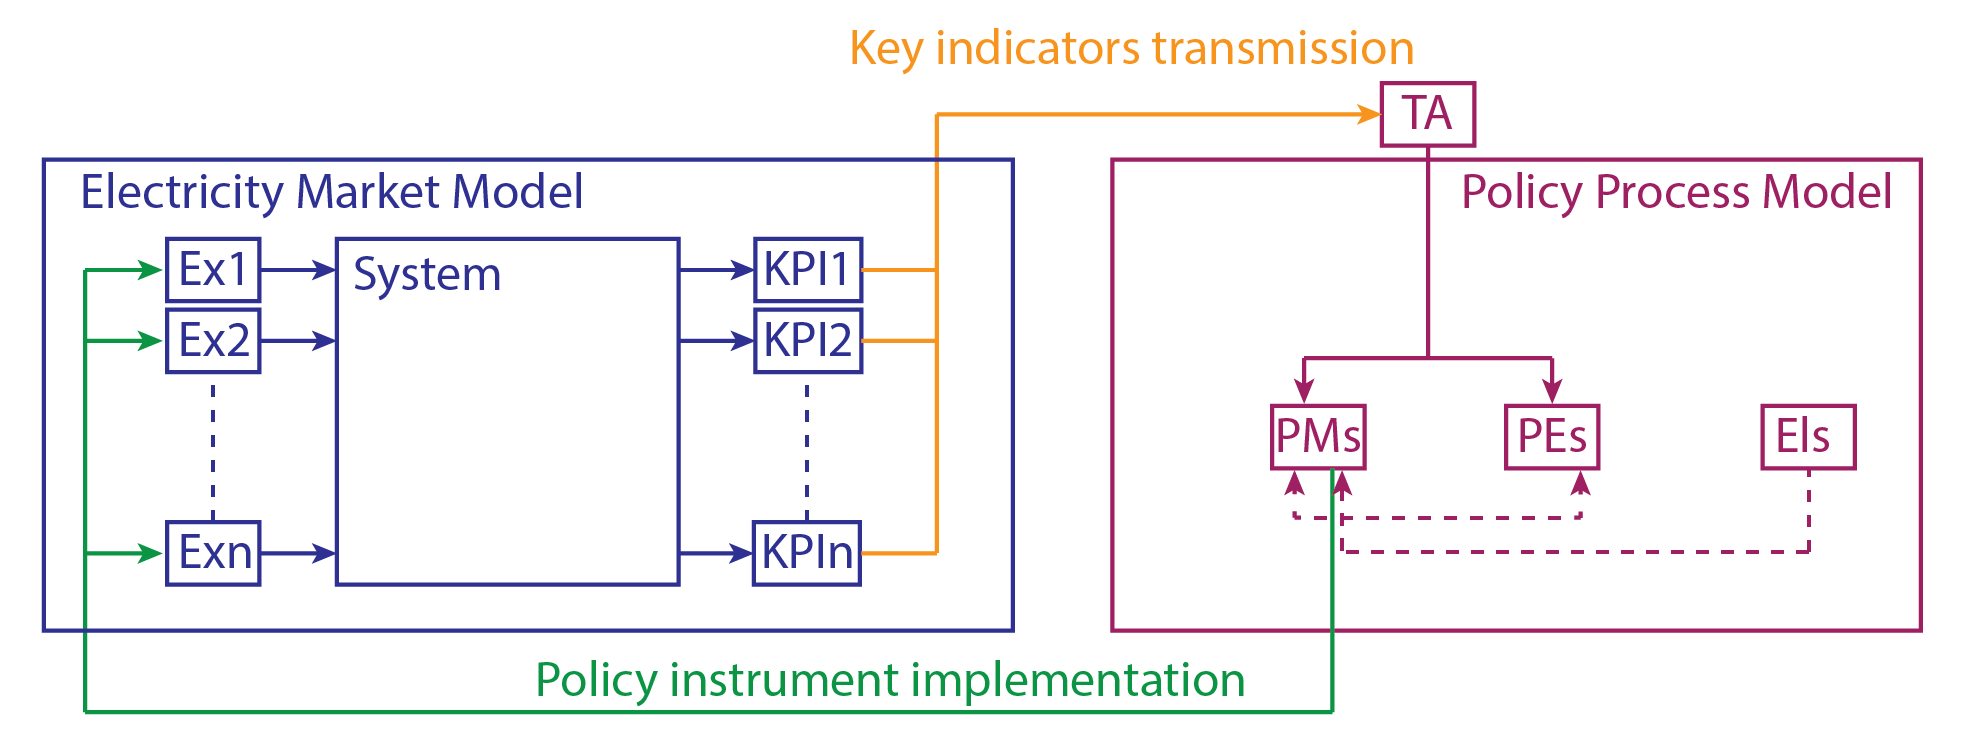
\includegraphics[width=\linewidth, keepaspectratio]{figures/ModuleInterface-09}
\caption{Diagram of the hybrid model.}
\label{fig:ModuleInterface-09}
\end{figure}

%%%%%%%%%%%% end of subsection

%%%%%%%%%%%%
\subsection{The problem tree}
\label{ssec:interfaceProblemTree}

To couple the models, the agents in the policy process need to be provided with a problem tree. This problem tree is specific to the electricity market model as it is informed by the key performance indicators from that model. This was highlighted in the previous section. Beyond this, the problems selected are also informed from previous work done by \cite{markard2016socio}. They identified a number of problems (they call these beliefs in their publication) that are specific to the Swiss context. These are however limited to the deep core and policy core levels. Secondary problems are not included or researched and are therefore taken from the model only.

The difficulty in the creation of the problem tree is to associate the right indicators to the right problems. The first step is to not consider the deep core problems. These are considered to be normative problems. They are beyond the boundaries of the model, out of the scope. They are not a crucial aspect of the process as it is focused on policy core problems so it does not make a big difference if deep core problems are considered or not. The next step is to consider the secondary problems. These can be found directly within the model. They are indicators that are made into secondary problems. Not all indicators are considered, only a few are selected. These are considered to be the important ones for the agents in the policy process. Finally, there is the selection of the policy core problems. These are, in general, aggregates of the secondary problems. They are calculated as a function of the main model indicators.

For the policy core problems, there is an additional aspect that needs to be considered. In work performed by \citeauthor{markard2016socio}, policy core problems within the Swiss electricity market subsystem were identified. These are: seriousness of the problem, role of the state, environment, economy and society. Several of these cannot be obtained from the model as they are outside of the boundaries of the model. However, the environment and economy can be considered. They are therefore selected as the policy core problems. \cite{markard2016socio} also identified four secondary problems. They are however not suitable for the model as they are more questions than problems. Furthermore, four secondary problems is not sufficient. It is for this reason that the secondary problems are only selected from the model. Ultimately, the policy core problems are calculated using linear equations that include a number of the indicators used for the secondary problems.

Overall, the problem tree is given as follows:

\begin{itemize}
\item Policy core problems:
	\begin{itemize}
	\item Economy
	\item Environment
	\end{itemize}
\item Secondary problems:
	\begin{itemize}
	\item Renewable energy production
	\item Nuclear production
	\item Fossil fuel production
	\item Amount of imports
	\item Amount of exports
	\item Electricity prices
	\item Investment levels
	\item Domestic emission levels
	\item Imported emission levels
	\end{itemize}
\end{itemize}

The economy takes into account elements related to profits of firms along with the security of supply of the country. The environment takes into account aspects such as the emissions, the amount of renewable energy and the amount of imported emissions.

%From markard2016socio, no deep core beliefs. Policy core beliefs are: seriousness of the problem, role of the state, environment, economy and society. In total, they identified 18 policy core beliefs. Most of these are beyond the scope of the model. The secondary beliefs identified are: phase out of nuclear, new nuclear plants, expansion of RES targets, expansion of energy demand targets, electricity suppliers role to fulfil efficiency targets.

%\begin{itemize}
%\item DC0 - Economy
%\item DC1 - Ecology
%\item PC0 - Security of supply
%\item PC1 - Profit levels - This is the average profits divided by the average revenues
%\item PC2 - Emissions - This is the average of domestic and imported emissions.
%\item S0 - Renewable energy production - This is calculated as the amount of renewable energy produced locally divided by the amount of energy produced overall.
%\item S1 - Nuclear production - This is the average production of nuclear over the total domestic production.
%\item S2 - Fossil fuel production - This is the average production of gas over the total domestic electricity production.
%\item S3 - Amount of imports
%\item S4 - Amount of exports - This is the average total amount of exports divided by the total demand
%\item S5 - Electricity prices - This is the price average. A maximum average price of 100 is assumed.
%\item S6 - Investment levels - This is the amount of investment (renovation + construction spent) over the amount of 
%\item S7 - Imported emission levels - This is the sum of all imported emissions from fossil fuel power plants divided by the total imported electricity. A maximum has to be found for normalisation based on average values.
%\end{itemize}

%%%%%%%%%%%% end of subsection

%%%%%%%%%%%%
\subsection{The policy instruments}
\label{ssec:interfaceInstruments}

The policy instruments within the policy tree are implemented using incremental increases and decreases in the following exogenous parameters.

\begin{enumerate}
\item Solar subsidies
\item Wind turbine permit times
\item Agent's hurdle rate
\item Carbon tax on fossil fuel imports
\item Carbon tax on domestic fossil fuel
\end{enumerate}

%%%%%%%%%%%% end of subsection

%%%%%%%%%%%%%%%%%%%%%%%%%%%%%%%%%%%%%%%%% end of section








